\section{Gaussian processes}


%%%%%%%%%%%%%%%%%%%%%%
\subsection{Introduction}
%%%%%%%%%%%%%%%%%%%%%%

\begin{frame}{What comes to $your$ mind when you hear ``Gaussian processes''?}
\end{frame}

\begin{frame}{Gaussian processes}
\begin{center}
	\only<1>{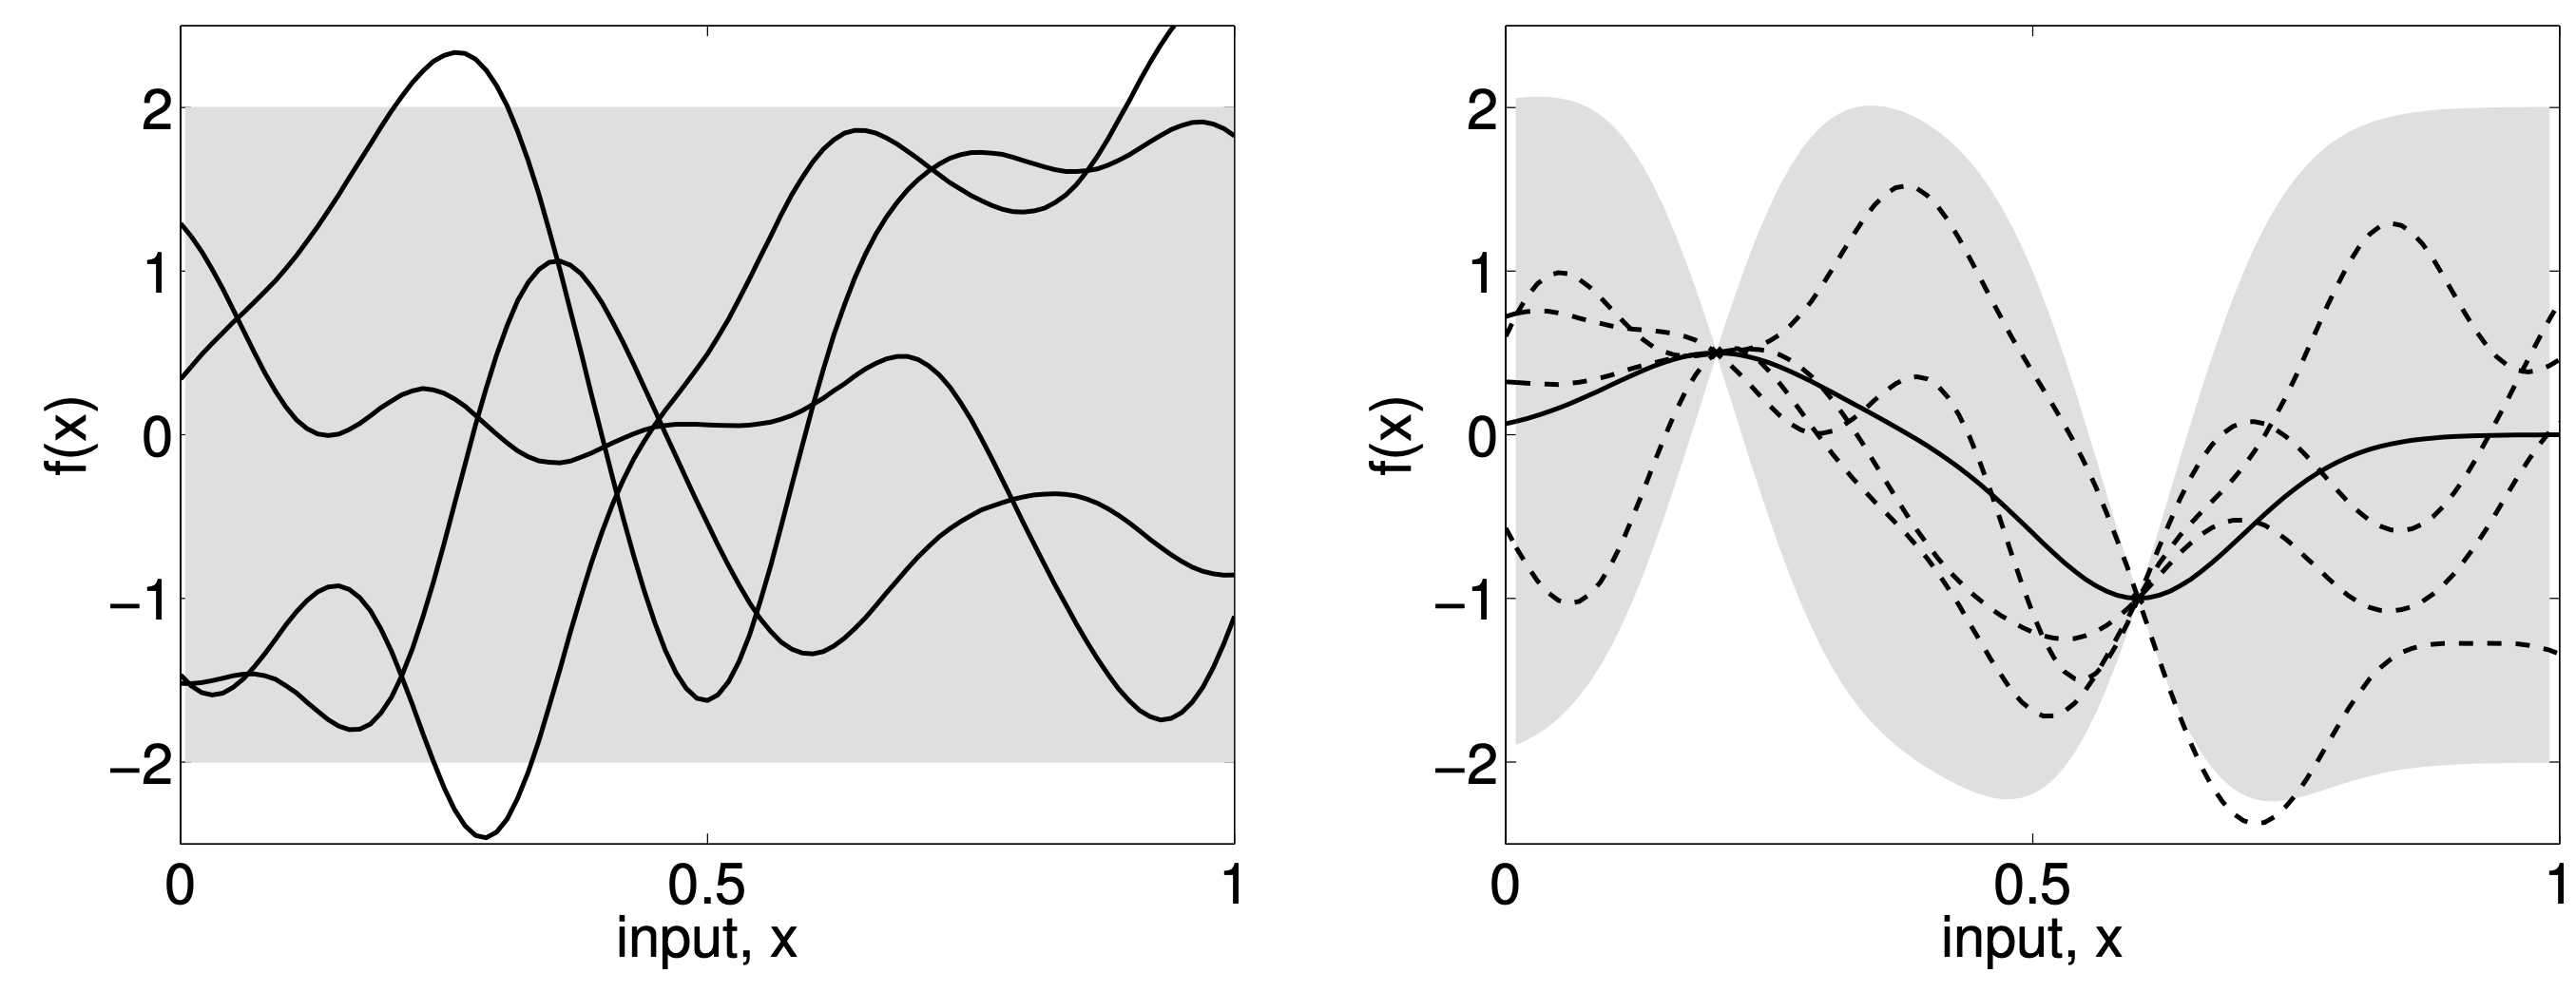
\includegraphics[height=.45\textheight]{figures_julyan/gp/gprw1}}
	\only<2>{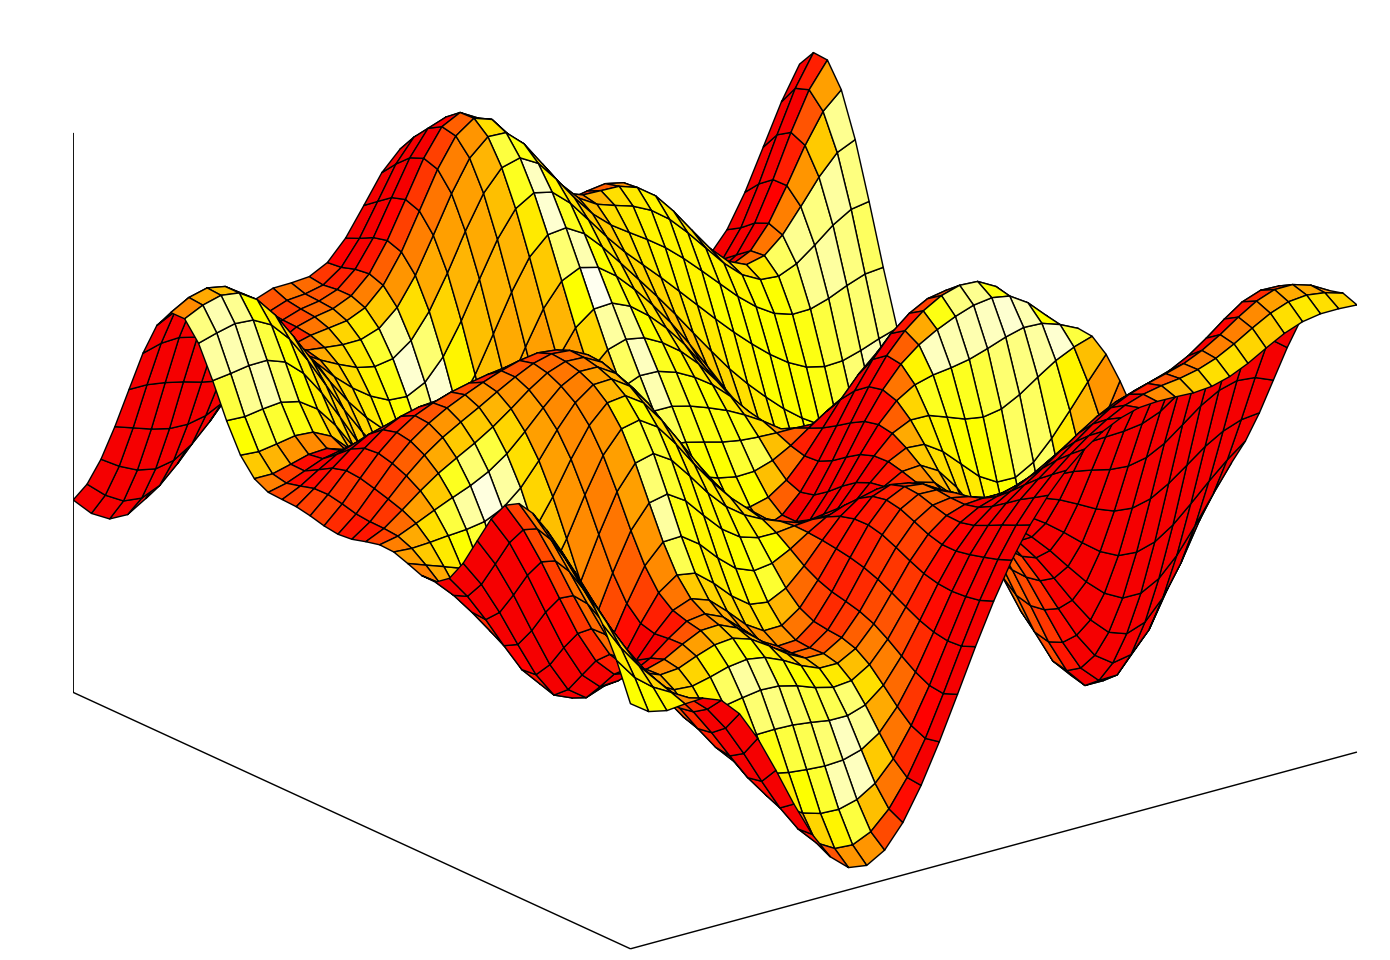
\includegraphics[height=.6\textheight]{figures_julyan/gp/gprw2}}
\end{center}
\hfill From \citet{Rasmussen:2006aa}
\end{frame}

\begin{frame}{Gaussian processes}
%\textcolor{gray}{What this chapter is about:}
%\begin{itemize}
%	\item How to use GPs in Bayesian inference
%	\item RKHS
%\end{itemize}\pause
%\textcolor{gray}{What this chapter is not about:}
%\begin{itemize}
%	\item Relationship with regularization theory, splines, support vector machines
%	\item PAC-Bayes analysis
%	\item Approximation methods: GP prediction methods is intractable for large sample $n$ datasets with complexity $\mathcal{O}(n^3)$ due to inversion of $n\times n$ matrix
%\end{itemize}\pause
\textcolor{gray}{Links with other chapters:}
\begin{itemize}
	\item GPs are used are \alert{BNP priors} on curves
	\item As such, the properties of the induced posterior are studied in the section on  \alert{asymptotics}
	\item Wide limit in  \alert{Bayesian neural networks}
	\item  \alert{SGD} with constant learning rate
	\item GPs are the nonparametric counterpart of the \alert{multivariate Gaussian distribution}, just like the \alert{Dirichlet process} is the nonparametric counterpart of the \alert{Dirichlet distribution}
\end{itemize}
\end{frame}


\begin{frame}{Gaussian process, Dirichlet process, and their parametric counterparts}
	\begin{center}
		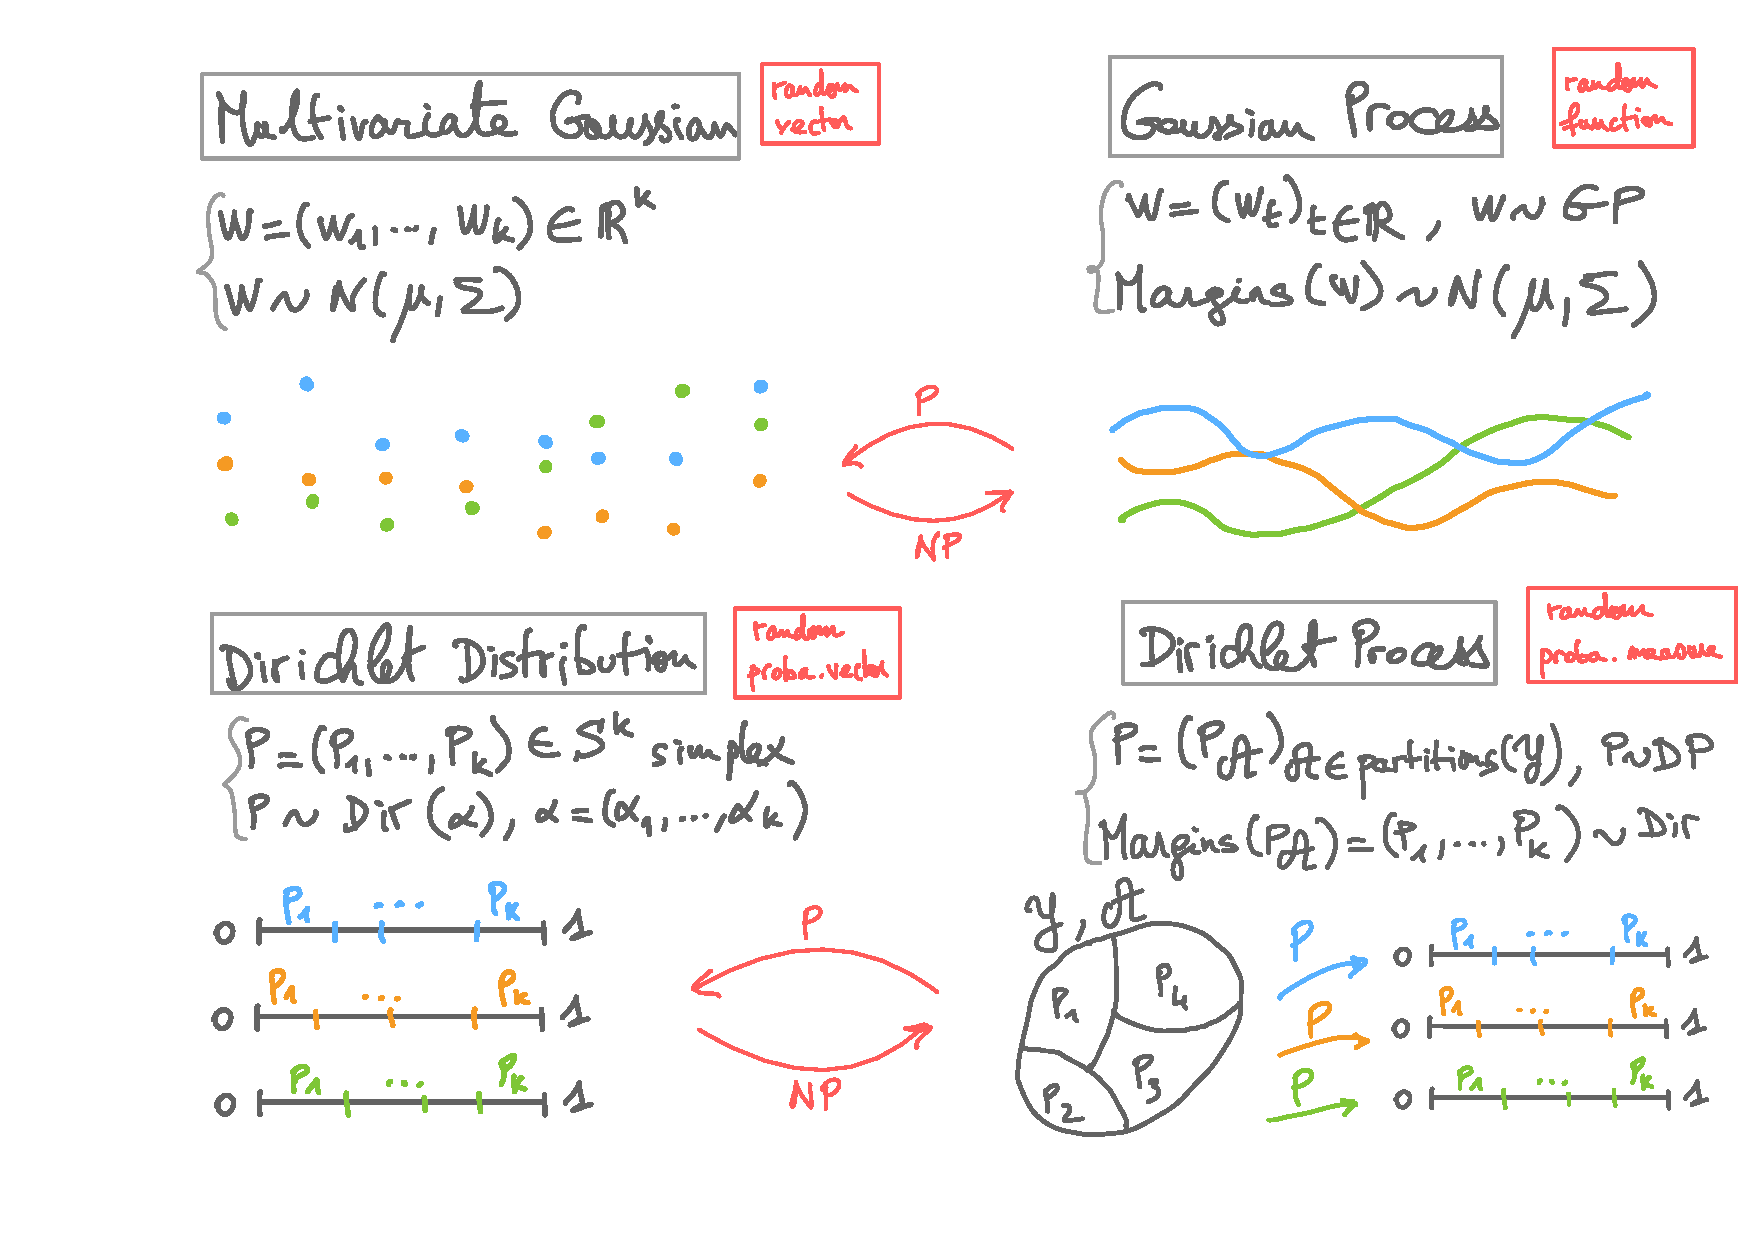
\includegraphics[width=\textwidth]{figures_julyan/gp/gp-and-dp.pdf}
	\end{center}
\end{frame}



\begin{frame}{References}
\begin{itemize}
	\item \alert{Main reference on GPs}: \fullcite{Rasmussen:2006aa}
	\item \alert{GPs in Bayesian inference}: Chapter 11 of \fullcite{ghosal2017fundamentals}
	\item \alert{Chapter 18} on Gaussian processes of \fullcite{murphy2023probabilisticMLadvanced}
\end{itemize}
\end{frame}




\begin{frame}{Supervized learning}

Two common approaches to \alert{supervized learning}:
\begin{itemize}
	\item restrict the class of functions considered, for example only linear functions of the input
	\item give a prior probability to every possible function, where higher probabilities are given to functions that we consider to be more likely
\end{itemize}

\end{frame}



\begin{frame}{Gaussian processes}
\begin{block}{Definition \citep{Rasmussen:2006aa}}
	A \alert{Gaussian process} is a collection of random variables, any finite number of which have a joint Gaussian distribution.
\end{block}

\pause

\begin{block}{Definition \citep{ghosal2017fundamentals}}
	A \alert{Gaussian process} is a stochastic process $W =(W_t: t \in T)$ indexed by an arbitrary set $T$ such that the vector $(W_{t_1},\ldots,W_{t_k})$ possesses a multivariate
normal distribution, for every $t_i\in T$ and $k\in \mathbb{N}$. A Gaussian process $W$ indexed by $\mathbb{R}^d$ is called:
\begin{itemize}
	\item  \alert{self-similar} of index $\alpha$ if $(W_{\sigma t}:t \in \mathbb{R}^d)$ is distributed like $(\sigma^\alpha W_{t}:t \in \mathbb{R}^d)$, for every $\sigma  > 0$, and 
	\item \alert{stationary} if $(W_{t+h}:t \in \mathbb{R}^d)$  has the same distribution of $(W_{t}:t \in \mathbb{R}^d)$, for every $h\in \mathbb{R}^d$.
\end{itemize}
\end{block}

\end{frame}



\begin{frame}{Mean function and covariance kernel}

Vectors $(W_{t_1},\ldots,W_{t_k})$ are called \alert{marginals}, and their distributions \alert{marginal distributions} or \alert{finite-dimensional distributions}

\pause


\begin{block}{Mean function and covariance kernel}
Finite-dimensional distributions are determined by the \alert{mean function} and \alert{covariance kernel}, defined by
$$\mu(t) = \E (W_t), \quad 
K(s, t) = \text{Cov}(W_s, W_t), \quad s, t \in  T.$$
\end{block}
\end{frame}



\begin{frame}{Scaling}

\begin{alertblock}{Scaling}
If $W =(W_t: t \in \mathbb{R}^d)$ is a Gaussian process  with covariance kernel $K$, then the process $(W_{\sigma t}: t \in \mathbb{R}^d)$ is another Gaussian process, with covariance kernel $K(\sigma s, \sigma t)$, for any $\sigma  > 0$. A scaling factor $\sigma  > 1$ shrinks the sample paths, whereas a factor $\sigma  < 1$ stretches them.
\end{alertblock}

\pause

\begin{center}
	\only<2>{
	$\sigma  > 1$ \hspace{4.5cm} $\sigma  < 1$ 
	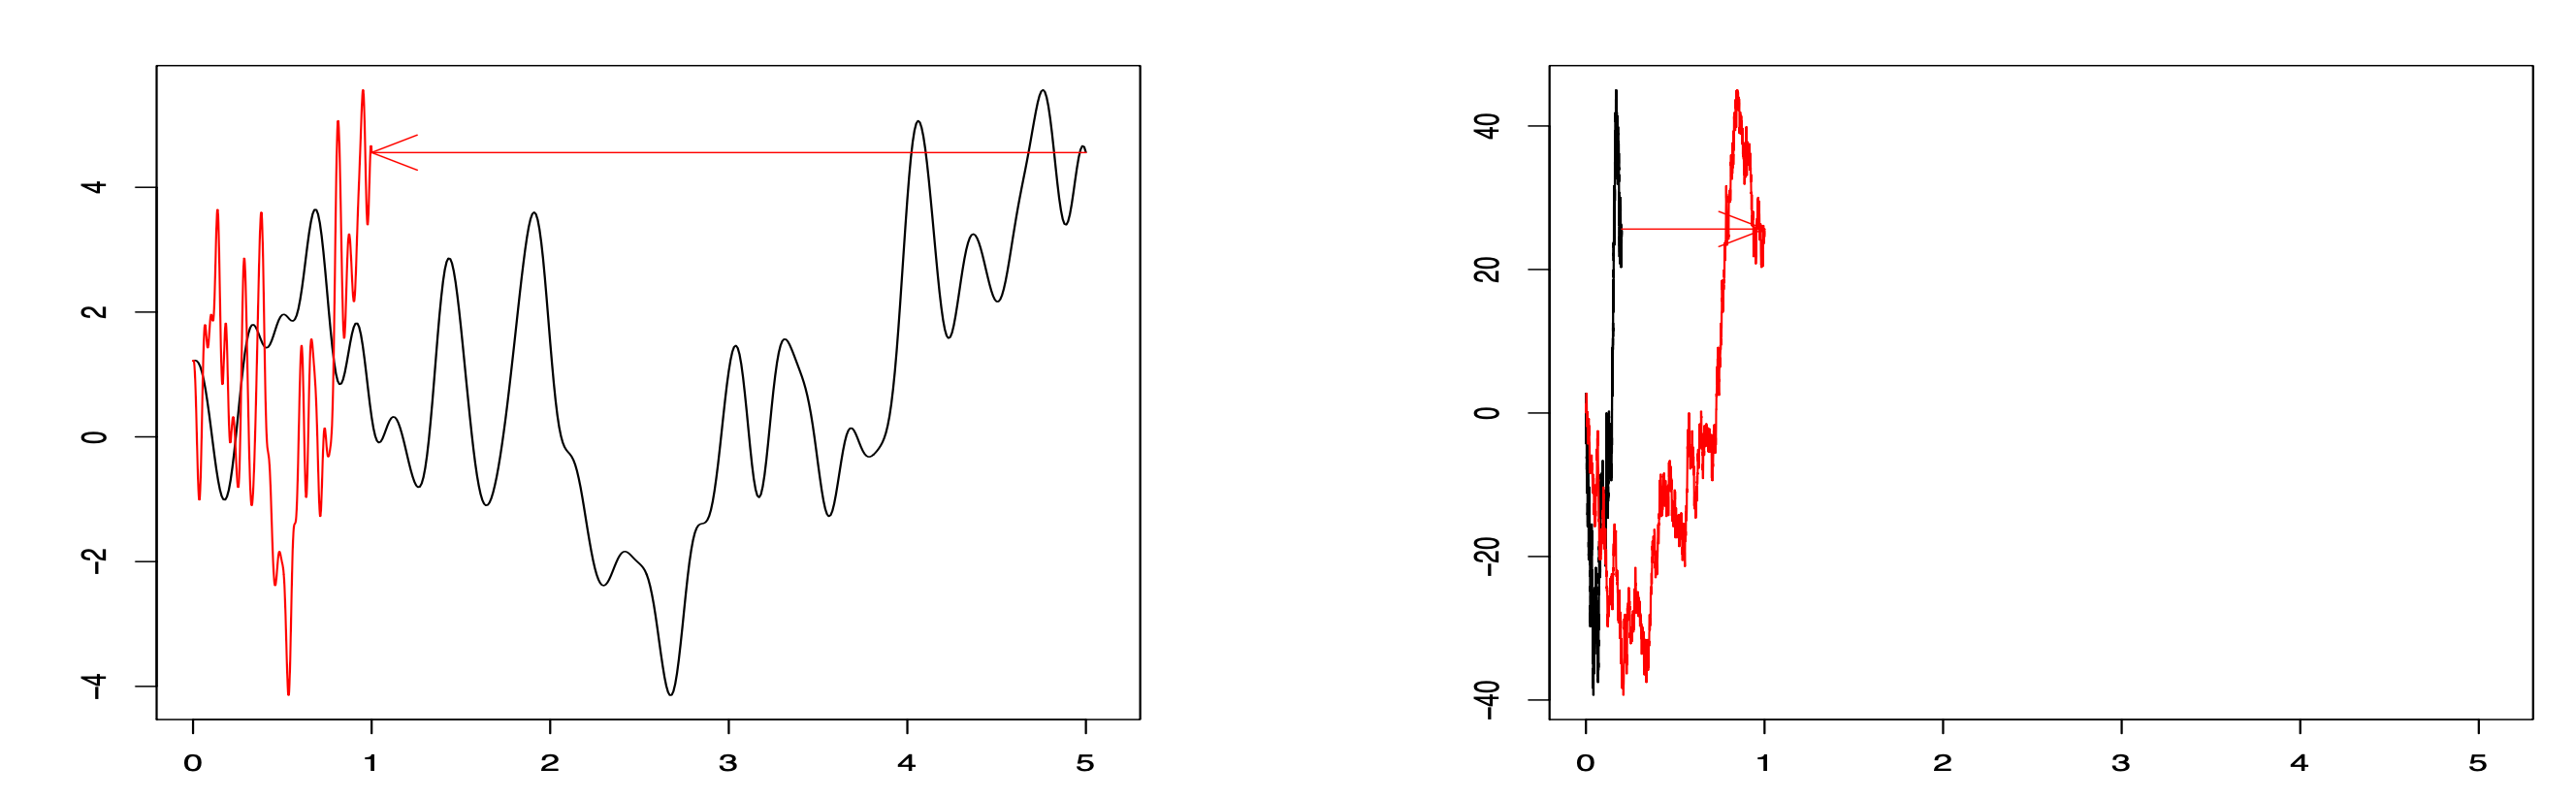
\includegraphics[height=.35\textheight]{figures_julyan/gp/scaling}
	}
\end{center}
\hfill From \citet{ghosal2017fundamentals}


\end{frame}


\subsection{Examples}


\begin{frame}{Examples}
\begin{exampleblock}{Random series}
	If $Z_1,\ldots,Z_m\simiid \mathcal{N}(0,1)$ and $a_1,\ldots,a_m$ are [deterministic] functions, then the \textit{Random series} $W_t = \sum_{i=1}^m a_i(t)Z_i$ defines a Gaussian process with:\bigskip
	
		\indent $\mu(t)=$\bigskip
		
		\indent $K(s, t)=$
%	\begin{align*}
%		\mu(t) & = \\
%		K(s, t) & = 
%	\end{align*}
\end{exampleblock}

\end{frame}


\begin{frame}{Examples}

\begin{exampleblock}{Brownian motion (or Wiener process)}
	The \textit{Brownian motion} is the zero-mean Gaussian process, say on $[0,\infty)$, with continuous sample paths and covariance function $K(s,t)=\min(s,t)$.
\end{exampleblock}

\pause


\begin{alertblock}{Brownian motion properties}
	Let $B_t$ be a Brownian motion, then $\forall s< t$:
	\begin{itemize}
		\item \alert{Stationarity}:  $B_t-B_s\sim \mathcal{N}(0,t-s)$
		\item \alert{Independent increments}:  $B_t-B_s \perp\!\!\!\!\perp (B_u, u\leq s)$
	\end{itemize}
	Thus it is a L\'evy process.
	\begin{itemize}
		\item \alert{Self-similar} of index $1/2$.
	\end{itemize}
\end{alertblock}

\end{frame}


\begin{frame}{Examples}

\begin{exampleblock}{Ornstein--Uhlenbeck}
	The standard \textit{Ornstein--Uhlenbeck process} with parameter $\theta>0$ is a mean-zero, stationary GP with time set $T = [0, \infty)$, continuous sample paths, and covariance function
		$$K(s,t) = (2\theta)^{-1}\exp\left(-\theta|t-s|\right).$$
\end{exampleblock}

\pause

\begin{alertblock}{Properties of Ornstein--Uhlenbeck process}
	The standard Ornstein--Uhlenbeck process with parameter $\theta>0$ can be constructed from a Brownian motion $B$ through the relation 	
	$$W_t = (2\theta)^{-1/2}\exp\left(-\theta t\right)B_{e^{2\theta t}}.$$
\end{alertblock}

\pause

Relationship between [fixed learning rate] \alert{stochastic gradient descent} (SGD) and \alert{Markov chain Monte Carlo} (MCMC) through the Ornstein--Uhlenbeck process: see \citet{mandt2017stochastic}.


\end{frame}


\begin{frame}{Examples}

	
\begin{exampleblock}{Square exponential}
	GP with covariance function (a.k.a. radial basis function kernel)
	$$K(s,t) = \exp\left(-\frac{\Vert t-s\Vert^2}{2\ell^2}\right).$$
	Parameter $\ell$ is called the \textit{characteristic length-scale}.
\end{exampleblock}


\begin{exampleblock}{Fractional Brownian motion}
	The \textit{fractional Brownian motion} (fBm) with \textit{Hurst parameter} $\alpha\in  (0, 1)$ is the mean zero Gaussian process $ W = (W_t : t \in  [0, 1])$ with continuous sample paths and covariance function
	$$K(s,t) = \frac{1}{2}\left(s^{2\alpha}+t^{2\alpha}-|t-s|^{2\alpha}\right).$$
	\begin{itemize}
		\item $\alpha=1/2$ yields the standard Brownian motion.
	\end{itemize}
\end{exampleblock}
	
\end{frame}


\begin{frame}{Practical}
\begin{alertblock}{Practical}
	\ComputerMouse\,\, Try practical on Gaussian process sampling,  \alert{gaussian-process-sampling.ipynb}.
\end{alertblock}
\end{frame}

\subsection{Gaussian process regression}


\begin{frame}{Conditional distributions of a multivariate Gaussian}
Let an $N$-dimensional Gaussian vector $\mathbf {x}$  be partitioned as:\\  
$\mathbf {x}={\begin{bmatrix}\mathbf {x} _{1}\\\mathbf {x} _{2}\end{bmatrix}}$ with sizes $q$ and $N-q$, and accordingly ${\boldsymbol {\mu }}$ and ${\boldsymbol \Sigma}$ are partitioned as
${\boldsymbol {\mu }}={\begin{bmatrix}{\boldsymbol {\mu }}_{1}\\{\boldsymbol {\mu }}_{2}\end{bmatrix}}$ with sizes $q$ and $N-q$ and 
$${\displaystyle {\boldsymbol {\Sigma }}={\begin{bmatrix}{\boldsymbol {\Sigma }}_{11}&{\boldsymbol {\Sigma }}_{12}\\{\boldsymbol {\Sigma }}_{21}&{\boldsymbol {\Sigma }}_{22}\end{bmatrix}}{\text{ with sizes }}{\begin{bmatrix}q\times q&q\times (N-q)\\(N-q)\times q&(N-q)\times (N-q)\end{bmatrix}}}.$$
Then 
\begin{itemize}
	\item the \alert{conditional distribution} of $ \mathbf x_1$, conditioned on $\mathbf x_2 = a$, is multivariate normal $\mathcal{N}_q( \bar{ \boldsymbol {\mu} }, \bar{ \boldsymbol {\Sigma} })$ where
${ {\bar {\boldsymbol {\mu }}}={\boldsymbol {\mu }}_{1}+{\boldsymbol {\Sigma }}_{12}{\boldsymbol {\Sigma }}_{22}^{-1}\left(\mathbf {a} -{\boldsymbol {\mu }}_{2}\right)}$
and 
${ {\bar {\boldsymbol {\Sigma }}}={\boldsymbol {\Sigma }}_{11}-{\boldsymbol {\Sigma }}_{12}{\boldsymbol {\Sigma }}_{22}^{-1}{\boldsymbol {\Sigma }}_{21}}$;
	\item the \alert{marginal (unconditional) distribution} of $ \mathbf x_1$ is multivariate normal $\mathcal{N}_q( \boldsymbol {\mu}_1, \boldsymbol {\Sigma }_{11})$.
\end{itemize}

\end{frame}


\begin{frame}{Gaussian process regression without noise}
	Let a regression function modeled by a Gaussian process as follows:
%
\begin{equation*}
       \mathbf{f} \, \lvert\, \mathbf{X} \sim GP(\mathbf{f} \, \lvert\, \boldsymbol\mu, \mathbf{K}), 	
\end{equation*}
where $\mathbf{X} = [\mathbf{x}_1, \ldots, \mathbf{x}_n ]$ represents the observed data points, $\mathbf{f} = \left[ f(\mathbf{x}_1), \ldots, f(\mathbf{x}_n) \right]$ the function values, $\boldsymbol\mu = \left[ m(\mathbf{x}_1), \ldots, m(\mathbf{x}_n) \right]$ the mean function, and $K_{ij} = k(\mathbf{x}_i,\mathbf{x}_j)$ the kernel function. Assume $\boldsymbol\mu=0$. We want to predict $\mathbf{f}(\mathbf{X}_*)$ at new points $\mathbf{X}_*$. The joint distribution of $\mathbf{f}$ and $\mathbf{f}_*$ is expressed as:
%
    \begin{align}
       \begin{bmatrix}\mathbf{f} \\ \mathbf{f}_*\end{bmatrix} \sim \mathcal{N}\left(\mathbf{0}, \begin{bmatrix}\mathbf{K} & \mathbf{K}_* \\ \mathbf{K}_*^\mathsf{T} & \mathbf{K}_{**}\end{bmatrix}\right), \nonumber
    \end{align}
%
where $\mathbf{K}=K(\mathbf{X}, \mathbf{X})$, $\mathbf{K}_* = K(\mathbf{X}, \mathbf{X}_*)$ and $\mathbf{K}_{**}=K(\mathbf{X}_*, \mathbf{X}_*)$. The conditional distribution of interest is:
\begin{align}
       \mathbf{f}_* \, \vert \, \mathbf{f}, \mathbf{X}, \mathbf{X}_* \sim \mathcal{N} \left(\mathbf{K}_*^\mathsf{T} \, \mathbf{K}^{-1} \, \mathbf{f}, \: \mathbf{K}_{**} - \mathbf{K}_*^\mathsf{T} \, \mathbf{K}^{-1} \, \mathbf{K}_* \right). \nonumber
    \end{align}
\end{frame}


\begin{frame}{Gaussian process regression with noise}
Oftentimes, we only have access to noisy versions of the true function, $y = f(x) + \epsilon$, where $\epsilon$ represents additive i.i.d. Gaussian noise with variance $\alert{\sigma^2}$. Then $\text{cov}(y) = \mathbf{K} + \alert{\sigma^2} \mathbf{I}$. The joint distribution of the observed values and the function values at new testing points is:
%
    \begin{align}
       \begin{pmatrix}\mathbf{y} \\ \mathbf{f}_*\end{pmatrix} \sim\mathcal{N}\left(\mathbf{0}, \begin{bmatrix}\mathbf{K} + \alert{\sigma^2} \mathbf{I} & \mathbf{K}_* \\ \mathbf{K}_*^\mathsf{T} & \mathbf{K}_{**}\end{bmatrix}\right) \ . \nonumber
    \end{align}
%
Using the conditional distribution, we now get:
%
    \begin{align}
       \mathbf{{f}_*} \, \vert \, \mathbf{X}, \mathbf{y}, \mathbf{X}_* \sim \mathcal{N} \left(\mathbf{K}_*^\mathsf{T} [\mathbf{K} + \alert{\sigma^2} \mathbf{I}]^{-1} \mathbf{y}, \mathbf{K}_{**} - \mathbf{K}_*^\mathsf{T} [\mathbf{K} + \alert{\sigma^2} \mathbf{I}]^{-1} \mathbf{K}_*\right). \nonumber
    \end{align}	
\end{frame}

\begin{frame}{Practical}
\begin{alertblock}{Practical}
	\ComputerMouse\,\, Try practical on Gaussian process regression,  \alert{gaussian-process-regression.ipynb}.
\end{alertblock}
\end{frame}


%
%\begin{frame}{Kriging}
%
%\begin{exampleblock}{Kriging}
%	For a given Gaussian process $W = (W_t : t \in T)$ and fixed, distinct points $t_1,\ldots,t_m \in T$, the conditional expectations $W_t^\star  = \E [ W_t|W_{t_1},\ldots,W_{t_m}]$ define another Gaussian process.
%\end{exampleblock}
%
%\pause 
%
%\begin{block}{Exercise}
%	Find the covariance function of $W_t^\star$, say $K^\star(t,s)$, as a function of $(t_1,\ldots,t_m)$.
%\end{block}
%
%\pause 
%
%\begin{alertblock}{Properties of Kriging}
%	\begin{itemize}
%		\item If $W$ has continuous sample paths, then so does $W^\star$. 
%		\item In that case the process $W^\star$ converges to $W$ when $m \to \infty$  and the interpolating points $(t_1,\ldots,t_m)$ grow dense in $T$.
%	\end{itemize}
%\end{alertblock}
%\end{frame}

\subsection{Reproducing kernel Hilbert space}

\begin{frame}{Reproducing kernel Hilbert space}
	To every Gaussian process corresponds a Hilbert space, determined by its covariance kernel. This space determines the support and shape of the process, and therefore is crucial for the properties of the Gaussian process as a prior. 

\pause

Let's break down what each part means:

\alert{Reproducing Kernel}: This refers to a mathematical function that takes in two inputs and calculates a measure of similarity or distance between them. It's called \alert{reproducing} because it has a special property related to the inner product (a mathematical operation) that allows it to reproduce functions.

\alert{Hilbert Space}: This is a mathematical concept from functional analysis, which is basically a fancy way of saying a space where functions live. A Hilbert space is a mathematical structure that generalizes the notion of Euclidean space to infinite-dimensional spaces (formal def: inner product space that is complete wrt the distance function induced by the inner product).

%\pause
%
%\begin{block}{Definition}
%	A \textit{Hilbert space} is an inner product space that is complete wrt the distance function induced by the inner product.
%\end{block}
\end{frame}


\begin{frame}{Reproducing kernel Hilbert space}
For a Gaussian process $W = (W_t : t \in T)$, let $\overline{\text{lin}}(W)$ be the closure of the set of all linear combinations $\sum_I \alpha_i W_{t_i}$ in the $L_2$-space of square-integrable variables. The space $\overline{\text{lin}}(W)$ is a Hilbert space.

\pause

\begin{block}{Definition} 
The \textit{reproducing kernel Hilbert space} (RKHS) of the mean-zero, Gaussian process $W = (W_t : t \in T )$ is the set $\mathbb{H}$ of all functions $z_H:T \to \mathbb{R}$ defined by $z_H(t) = \E(W_t H)$, for $H$ ranging over $\overline{\text{lin}}(W)$. The corresponding inner product is
	$$\langle z_{H_1},z_{H_2}\rangle_{\mathbb{H}} =  \E (H_1H_2).$$
\end{block}
\end{frame}


\begin{frame}[allowframebreaks]{Reproducing kernel Hilbert space}

\begin{alertblock}{Properties of RKHS}
	\begin{itemize}
		\item Correspondance $z_H \leftrightarrow H$ is an isometry (by def of inner product), so the definition is well-posed (the correspondence is one-to-one), and $H$ is indeed a Hilbert space.
		\item Function corresponding to $H=\sum_I \alpha_i W_{s_i}$ is \bigskip
			$z_H=$
		\item For any $s\in T$, function $K(s,\cdot)$ is in RKHS $\mathbb{H}$ associated with $H = W_s$.
	\end{itemize}
\end{alertblock}

\framebreak

\begin{alertblock}{Reproducing formula}
For a general function $z_H \in \mathbb{H}$ we have $$\langle z_H, K(s, \cdot)\rangle_{\mathbb{H}} = \E (H W_s) = z_H(s).$$
That is to say, for any function  $h \in \mathbb{H}$,
	$$h(t) = \langle h, K(t, \cdot)\rangle_{\mathbb{H}}.$$
\end{alertblock}

\end{frame}

\begin{frame}{Example of RKHS: Euclidean space}
Let's consider a simple \alert{Euclidean space}, such as  $\mathbb{R}$. In this case, the RKHS corresponds to a space of functions defined on this real line.

Consider a set of data points on the real line, represented by pairs \((x_i, y_i)\) where \(x_i\) are the input values and \(y_i\) are the corresponding output values.

Let's model this data with a function \(f(x)\). In an RKHS framework, we can express this function as a linear combination of \alert{basis functions} \(k(x, x_i)\), where \(k\) is a  \alert{kernel function} that measures the similarity between input points \(x\) and \(x_i\).

The RKHS then consists of all functions that can be expressed as:
%
\[f(x) = \sum_{i=1}^{n} \alpha_i k(x, x_i)\]
%
where \(\alpha_i\) are coefficients that determine the weighting of each basis function.

Common choices for the kernel function in this context might be the linear kernel \(k(x, x_i) = x \cdot x_i\), the polynomial kernel \(k(x, x_i) = (x \cdot x_i + c)^d\), or the Gaussian kernel \(k(x, x_i) = \exp(-\|x - x_i\|^2 / 2\sigma^2)\).

The RKHS provides a flexible framework for modeling functions in this space using different kernel functions, allowing us to capture various types of relationships between input and output data points.\end{frame}

